La predicción del éxito o fracaso de las ubicaciones de puntos de acceso interior en diferentes planos utilizando conjuntos de datos con estructuras similares a la del presente trabajo se abordará a continuación en esta sección. En cada uno se describen el problema y su propósito, la metodología utilizada, las técnicas empleadas y los resultados.

\cite{pr_contreras2021modelwlan} publicaron el modelo de optimización  \citetitle{pr_contreras2021modelwlan} para el departamento de Investigación e Innovación en Ingenierías de la Universidad Simón Bolívar.

Debido a su movilidad y bajo costo, la demanda de redes inalámbricas, particularmente WLAN, ha aumentado significativamente. Para que estas redes inalámbricas funcionen en hogares, oficinas y escuelas, los puntos de acceso (AP) son necesarios. La ubicación y densidad de los AP tienen un impacto en la cobertura y la calidad de la señal. Para mejorar la eficiencia y la cobertura de la red, este artículo propone un modelo de optimización para la ubicación de AP en interiores que utiliza el modelo de propagación Log-Normal Shadowing Path Loss.

El desarrollo del modelo de optimización incluyó una serie de pasos importantes: se utilizó el modelo de propagación Log-Normal Shadowing Path Loss para estimar el radio de cobertura y la probabilidad de corte de la señal utilizando dimensiones del escenario, frecuencia y condiciones ambientales; se implementó un pseudocódigo para calcular el radio de cobertura y la probabilidad de corte de la señal para las bandas de 2,4 GHz y 5 GHz; y se diseñó una técnica específica para determinar la ubicación óptima de los AP dentro de una construcción, considerando la probabilidad de corte, la sensibilidad de recepción y otros parámetros técnicos.

Los resultados del modelo sugerido demostraron una mejora significativa en la identificación de las áreas de cobertura y la probabilidad de corte. En particular, se descubrió que la banda de 2.4 GHz cubre un mayor área de cobertura en comparación con la banda de 5 GHz, pero también se observó que tiene una mayor probabilidad de interferencia. La técnica permitió el cálculo de los radios de cobertura apropiados y la mejora de la ubicación geográfica de los AP, lo que permitió maximizar la cobertura y reducir las zonas de silencio. Las tablas y los gráficos que muestran la relación entre la distancia y la potencia de la señal describieron los parámetros específicos para cada banda de frecuencia y tipo de entorno.

El modelo de optimización para la ubicación de puntos de acceso en redes WLAN en ambientes interiores demostró ser efectivo para aumentar la cobertura y reducir la probabilidad de corte de señal como se ilustra en la Figura 3. Los algoritmos y metodologías creados ofrecen una herramienta útil para diseñar y desplegar redes WLAN de manera eficiente. Este modelo debería ser utilizado en futuras investigaciones y aplicaciones prácticas para mejorar la calidad y el rendimiento de las redes inalámbricas, especialmente en entornos con alta densidad de usuarios y dispositivos.

\begin{figure}[!ht]
	\begin{center}
		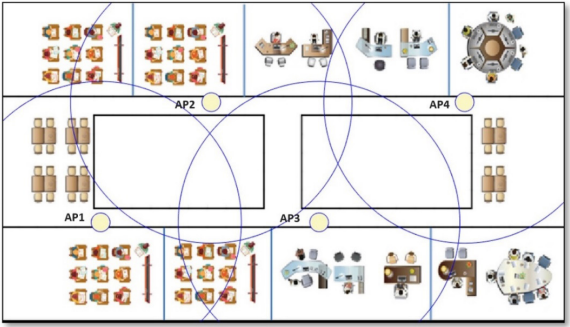
\includegraphics[width=0.80\textwidth]{2/figures/contreras2021.png}
		\caption[Diagrama de cobertura y ubicación de AP]{Diagrama de cobertura y ubicación de AP.\\
			Fuente: \cite{pr_contreras2021modelwlan}. \citetitle{pr_contreras2021modelwlan}. (p. 14)}
		\label{2:fig111}
	\end{center}
\end{figure}

Según el acta de la conferencia "2019 42nd International Conference on Telecommunications and Signal Processing (TSP)", que tuvo lugar en Budapest, Hungría, del 1 al 3 de julio de 2019, \cite{pr_ahmed2019impactaps} publicaron el artículo conocido como \citetitle{pr_ahmed2019impactaps}, "El impacto de la ubicación de los puntos de acceso en los sistemas de posicionamiento en interiores: un enfoque basado en la probabilidad", según su traducción al español.

La ubicación de los puntos de acceso (AP) en las redes WLAN es crucial para la estimación de la posición de los usuarios en los sistemas de posicionamiento internos. Este paper examina cómo la localización de AP afecta la precisión de las estimaciones de ubicación utilizando un método basado en probabilidades. Para evaluar el impacto de la ubicación de los AP en la probabilidad de una estimación correcta, se presentan tanto expresiones analíticas como resultados numéricos.

El estudio sigue una serie de pasos metodológicos: se crea un modelo de sistema de posicionamiento, se explica el algoritmo de estimación de la probabilidad correcta y se utiliza un enfoque analítico para calcular la probabilidad. Para evaluar el rendimiento, se implementan escenarios de colocación de AP y se realizan experimentos computacionales. Finalmente, se comparan los resultados de la probabilidad de estimación correcta bajo variaciones de ruido y diferentes ubicaciones de AP.

Los resultados indican que la ubicación de los AP tiene un impacto significativo en la probabilidad de una estimación precisa de la posición del usuario. La probabilidad máxima de estimación correcta para la mejor configuración de AP fue de alrededor de 0.92 en un escenario con desviación estándar de ruido ($\sigma$) igual a 1.5, mientras que la probabilidad máxima de estimación correcta para la configuración menos óptima fue de 0.64. Este aumento en la probabilidad se debe a que cada AP tiene una mayor área de cobertura en su configuración ideal como se puede observar en la Figura 4.

\begin{figure}[!ht]
	\begin{center}
		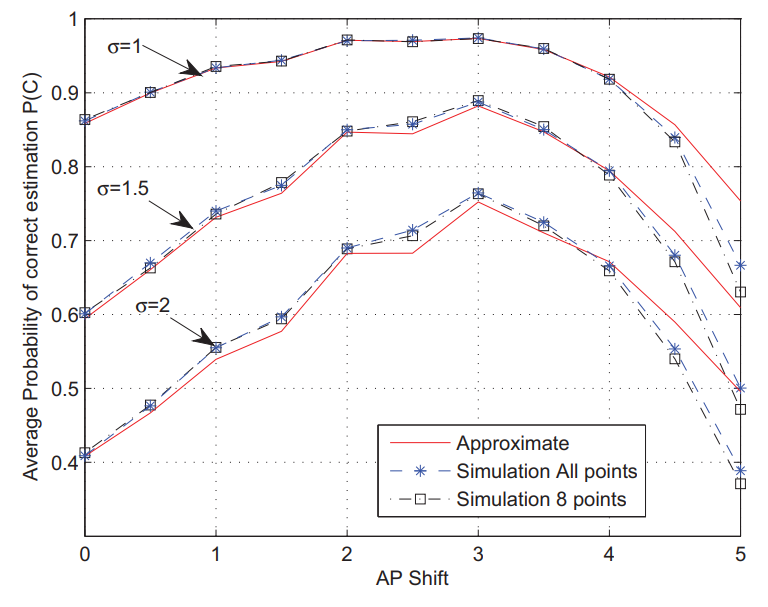
\includegraphics[width=0.80\textwidth]{2/figures/ahmed2019.png}
		\caption[Probabilidad media de estimación correcta en todos los puntos de la cuadrícula frente al desplazamiento de la distancia $\beta$ de los AP para $\sigma$ = {1, 1,5, 2}, expresión aproximada Ec. (12), resultados de la simulación todos los puntos y resultados de la simulación con 8 vecinos.]{Probabilidad media de estimación correcta en todos los puntos de la cuadrícula frente al desplazamiento de la distancia $\beta$ de los AP para $\sigma$ = {1, 1,5, 2}, expresión aproximada Ec. (12), resultados de la simulación todos los puntos y resultados de la simulación con 8 vecinos.\\
			Fuente: \cite{pr_ahmed2019impactaps}. \citetitle{pr_ahmed2019impactaps}. (p. 7)}
		\label{2:fig112}
	\end{center}
\end{figure}

Según el acta de la conferencia "TInternational Conference on Computational Science and Technology", que se llevó a cabo en 2022, \cite{pr_alathari2023optaps} publicaron el artículo conocido como \citetitle{pr_alathari2023optaps}, "Optimización de la ubicación de puntos de acceso en comunicaciones interiores" en español.

El estudio presenta un modelo de optimización para la ubicación de puntos de acceso (AP) en redes inalámbricas. Utilizando técnicas sofisticadas de algoritmos genéticos y simulaciones de Monte Carlo, el objetivo principal es maximizar la cobertura y minimizar la interferencia. La necesidad creciente de mejorar la eficiencia de las redes inalámbricas en entornos de alta densidad es el tema de esta investigación.

La técnica utilizada consta de numerosos pasos cruciales. Primero, se recopilan datos sobre la distribución del espacio y la cobertura. Después, se utiliza un algoritmo genético para crear las ubicaciones iniciales potenciales de AP. Se utilizan simulaciones de Monte Carlo para evaluar la efectividad de estas ubicaciones en términos de cobertura y minimización de interferencia. Se siguen estos pasos hasta llegar a la configuración de AP ideal.

Comparado con las técnicas convencionales, los resultados muestran una mejora significativa en la cobertura de la red y una reducción en la interferencia que se puede observar en la Figura 5. Se logró aumentar la cobertura en un 25 \% y disminuir la interferencia en un 15 \%. Estos hallazgos se comprobaron en un entorno simulado que emulaba las condiciones de una red inalámbrica de alta densidad real.

\begin{figure}[!ht]
	\begin{center}
		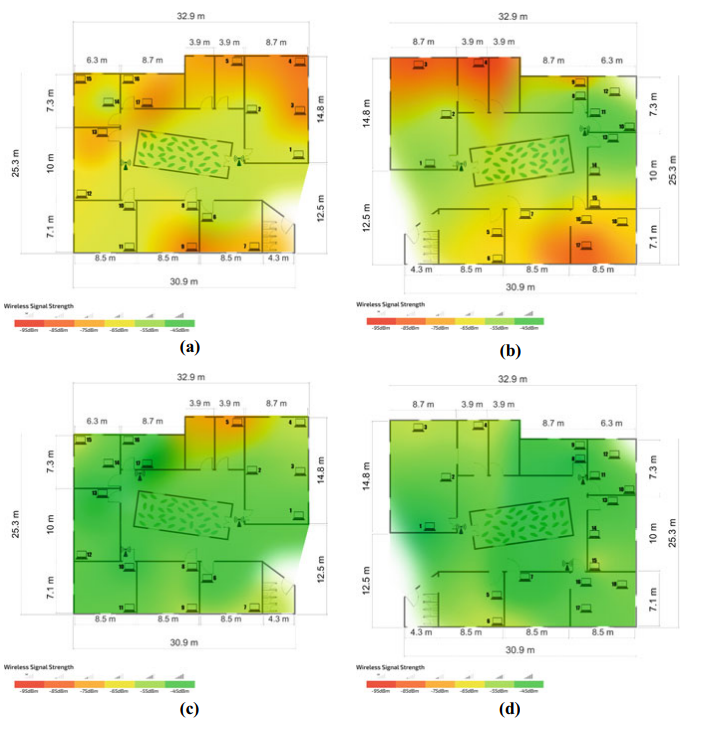
\includegraphics[width=0.75\textwidth]{2/figures/alathari2023.png}
		\caption[Un mapa de calor que describe la intensidad de la señal recibida antes y después. a Área de cobertura de la señal para los puntos de acceso de la izquierda, b Área de cobertura de la señal para los puntos de acceso de la derecha, c Área de cobertura de la señal para los puntos de acceso de la izquierda, d Área de cobertura de la señal para los puntos de acceso de la derecha.]{Un mapa de calor que describe la intensidad de la señal recibida antes y después. a Área de cobertura de la señal para los puntos de acceso de la izquierda, b Área de cobertura de la señal para los puntos de acceso de la derecha, c Área de cobertura de la señal para los puntos de acceso de la izquierda, d Área de cobertura de la señal para los puntos de acceso de la derecha.\\
		Fuente: \cite{pr_alathari2023optaps}. \citetitle{pr_alathari2023optaps}. (p. 11)}
		\label{2:fig113}
	\end{center}
\end{figure}

\clearpage
Según el acta de la conferencia "International Journal of Cyber and IT Service Management (IJCITSM)", que se llevó a cabo en Indonesia en 2022, \cite{pr_dudhat2022indoorwir} publicaron el artículo conocido como \citetitle{pr_dudhat2022indoorwir}, "Optimización del área de cobertura de redes inalámbricas de interior" en español.

Debido a las dificultades que presenta la propagación de ondas de radio en espacios cerrados, es crucial optimizar la cobertura de las redes inalámbricas en entornos interiores. Además, se pone de manifiesto que fenómenos como la dispersión, la reflexión y la refracción tienen un impacto en la calidad de las conexiones inalámbricas en interiores, lo que justifica el uso de modelos de propagación para mejorar la cobertura de la red.

El estudio utiliza una serie de procedimientos para maximizar el área de cobertura de la red inalámbrica interna. El número de puntos de acceso (APs) se determina utilizando la cobertura máxima de un AP y el área total a cubrir. Además, se utilizan modelos teóricos y empíricos para medir la fuerza de la red inalámbrica y se calcula el diámetro de los AP utilizando la fórmula MAPL (Pérdida Máxima Permitida).

Los resultados del estudio muestran que la eficiencia del canal y el porcentaje de actividad de los usuarios tienen un impacto significativo en la distribución de APs. Se puede calcular el número de APs necesarios para cubrir un área específica. Por ejemplo como se muestra en la Figura 6, se descubrió que para garantizar una cobertura óptima, se requieren alrededor de siete APs para una capacidad de usuario de 8 Mbps con un 164\% de actividad y una eficiencia del canal del 50%.

\begin{figure}[!ht]
	\begin{center}
		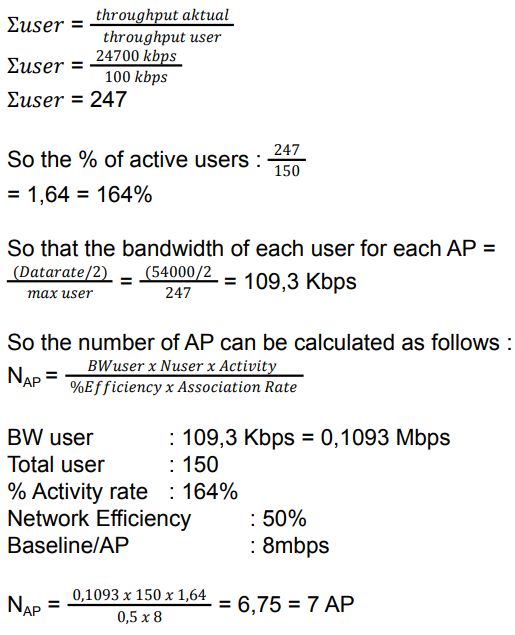
\includegraphics[width=0.5\textwidth]{2/figures/dudhat2022.png}
		\caption[La fórmula para determinar el número máximo de usuarios activos que puede suministrar un único AP, el número de AP, el ancho de banda de cada usuario para cada AP y el \% de usuarios activos]{La fórmula para determinar el número máximo de usuarios activos que puede suministrar un único AP, el número de AP, el ancho de banda de cada usuario para cada AP y el \% de usuarios activos.\\
			Fuente: \cite{pr_dudhat2022indoorwir}. \citetitle{pr_dudhat2022indoorwir}. (p. 11)}
		\label{2:fig114}
	\end{center}
\end{figure}

\newpage
\cite{pr_ketkhaw2019deepl}  publicaron la investigación \citetitle{pr_ketkhaw2019deepl}, en español "Predicción de la ubicación de puntos de acceso no autorizados basada en redes neuronales profundas", se publicó en el journal tailandés "Journal of Mobile Multimedia" en 2022.

El objetivo del estudio es desarrollar un método llamado LPRAP que utiliza redes neuronales profundas para predecir la ubicación de puntos de acceso no autorizados en redes inalámbricas locales. La detección y localización precisa de estos RAPs es esencial para garantizar la seguridad de las redes y proteger la información confidencial de posibles amenazas.

Los dos mecanismos principales del proceso LPRAP son la detección de RAPs y la predicción de su ubicación. Para determinar la intensidad de la señal recibida (RSSI) en cada subárea, se recopila un conjunto de marcos de balizas en la detección de RAP. Posteriormente, se clasifica la ubicación de los RAPs utilizando un espacio de características de 81 dimensiones. En cuanto a la predicción de ubicación, se utiliza la precisión de la predicción de ubicación para evaluar el rendimiento del esquema propuesto comparándolo con otros algoritmos de aprendizaje automático como SVM, KNN, Naive Bayes y MLP.

Los resultados del experimento muestran que LPRAP supera a todos los demás algoritmos de aprendizaje automático evaluados. La precisión de la predicción de la ubicación de los RAPs aumenta significativamente con el aumento del número de subáreas. Por ejemplo, LPRAP logra una precisión de predicción del 88,31\% para 3 subáreas, lo que demuestra su capacidad para detectar y encontrar RAPs en entornos de redes inalámbricas como se puede observar en la Figura 7.

\begin{figure}[!ht]
	\begin{center}
		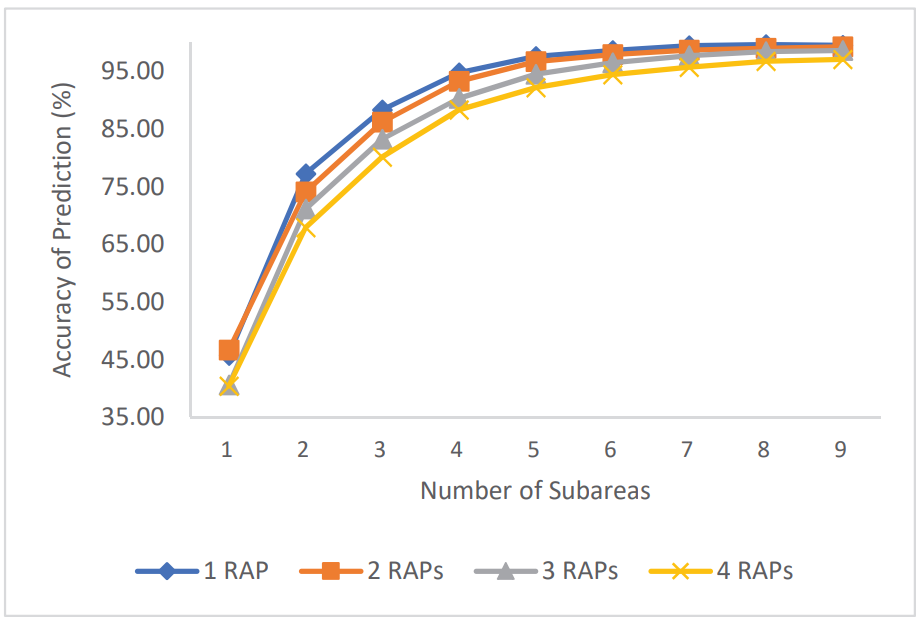
\includegraphics[width=0.75\textwidth]{2/figures/ketkha2022.png}
		\caption[Precisión de la predicción en función del número de subzonas para la predicción de la ubicación de 1 a 4 RAP.]{Precisión de la predicción en función del número de subzonas para la predicción de la ubicación de 1 a 4 RAP.\\
		Fuente: \cite{pr_ketkhaw2019deepl}. \citetitle{pr_ketkhaw2019deepl}. (p. 13)}
		\label{2:fig115}
	\end{center}
\end{figure}

\clearpage
En el acta de la conferencia "International Journal of Computing and Digital Systems" de 2021, que tuvo lugar en Bahrain, Indonesia, \cite{pr_mukti2021placemodelindo} publicó el artículo conocido como \citetitle{pr_mukti2021placemodelindo}. El término se traduce al español como "Modelo de colocación de puntos de acceso internos mediante Propagación Empírica Híbrida y Algoritmo Simulado de Recocido".

El estudio utiliza un método híbrido que combina modelos de propagación empírica y el algoritmo de Recocido Simulado (SA) para optimizar la ubicación de puntos de acceso (AP) en entornos interiores. El objetivo principal es mejorar la cobertura de la señal de AP, que es esencial para garantizar una conectividad efectiva en entornos inalámbricos.

El artículo proporciona una descripción detallada de la técnica, que incluye una serie de pasos cruciales. Inicialmente, se realiza una medición real de RSS en el campo a través de un estudio de sitio para recopilar información sobre la colocación de AP y los niveles de RSS en función de la distancia. Después, se implementa un modelo de dos dimensiones (2D) utilizando Visual Basic para calcular el área de cobertura utilizando un mapa de radio. Luego, se utiliza el algoritmo de Recocido Simulado para optimizar la ubicación de AP. Se toma en cuenta la función de costo, el esquema de enfriamiento, el mecanismo de inicialización de soluciones y el proceso de iteración.

Los resultados de la optimización de la ubicación de AP muestran mejoras significativas en la cobertura de área como se observa en la Figura 8. Por ejemplo, la cobertura del primer piso (lobby) aumentó del 66,851\% al 97,815\% después de la optimización. Similarmente, la cobertura en el tercer piso (sala de conferencias) aumentó del 88,368\% al 98,263\% después de aplicar el método propuesto. En todos los sitios de estudio, la cobertura de área aumentó en promedio un 19.202\%.

\begin{figure}[!ht]
	\begin{center}
		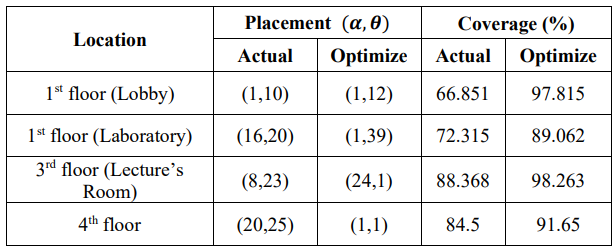
\includegraphics[width=0.95\textwidth]{2/figures/mukti2021.png}
		\caption[Colocación de Puntos de Acceso Y Optimización de la Cobertura]{Colocación de Puntos de Acceso Y Optimización de la Cobertura.\\
			Fuente: \cite{pr_mukti2021placemodelindo}. \citetitle{pr_mukti2021placemodelindo}. (p. 8)}
		\label{2:fig116}
	\end{center}
\end{figure}

\newpage
\cite{pr_nauata2021housegan} ,en la conferencia "2021 IEEE/CVF Conference on Computer Vision and Pattern Recognition (CVPR)", que tuvo lugar en Nashville, Tennessee, Estados Unidos en el año 2021, publicaron un artículo titulado \citetitle{pr_nauata2021housegan}, en español se traduce como "House-GAN++: Generative Adversarial Layout Refinement Network hacia un agente computacional inteligente para arquitectos profesionales".

Para la generación automatizada de planos de planta, se sugiere una red generativa rival de refinamiento de diseño de planos de planta (House-GAN++). El sistema recibe un diagrama de burbujas que muestra las conexiones funcionales entre las habitaciones y, como salida, crea un plano de planta realista.

Como se muestra en la Figura 9, la arquitectura sugerida integra una GAN relacional con restricciones de grafo y una GAN condicional. El generador itera el diseño antes de convertirlo en la siguiente restricción de entrada. Cada componente recibe una máscara de segmentación de la verdad fundamental con una probabilidad aleatoria durante el entrenamiento (condicionamiento GT por componente).

\begin{figure}[!ht]
	\begin{center}
		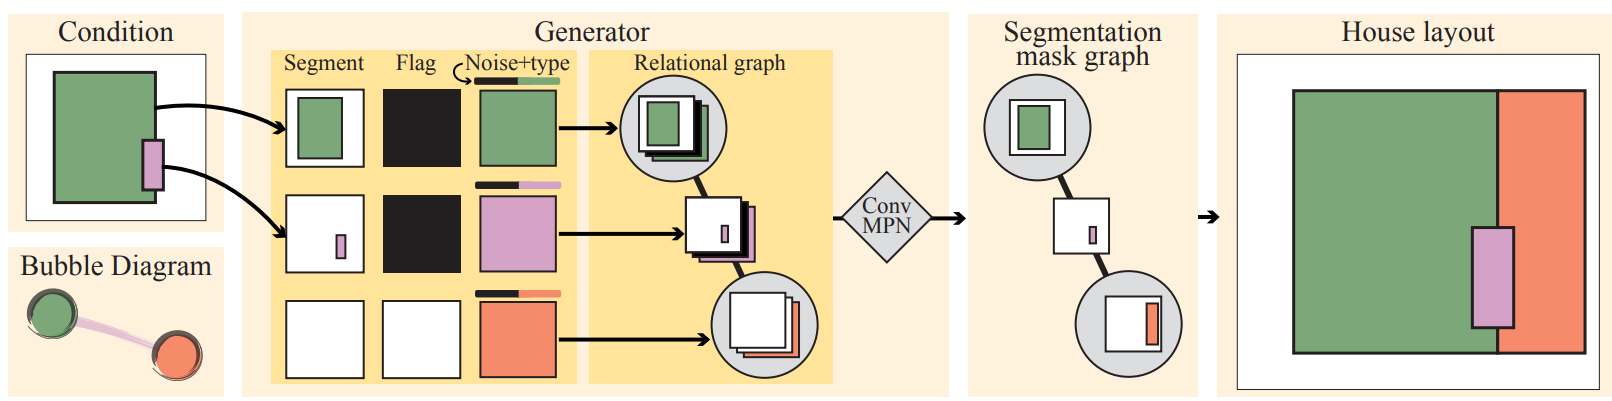
\includegraphics[width=0.8\textwidth]{2/figures/nauata2021.png}
		\caption[La arquitectura se basa en un GAN relacional. Se puede especificar una máscara de segmentación 2D adicional para cada habitación/puerta como condición de entrada, lo que permite un refinamiento iterativo del diseño.]{La arquitectura se basa en un GAN relacional. Se puede especificar una máscara de segmentación 2D adicional para cada habitación/puerta como condición de entrada, lo que permite un refinamiento iterativo del diseño.\\
		Fuente: \cite{pr_nauata2021housegan}. \citetitle{pr_nauata2021housegan}. (p. 3)}
		\label{2:fig117}
	\end{center}
\end{figure}

El sistema sugerido supera ampliamente los enfoques del estado del arte actuales en las tres métricas estándar de realismo, diversidad y compatibilidad. En un estudio de usuarios con arquitectos profesionales, el sistema obtuvo puntajes de realismo de -0.7 para los métodos comparativos y puntajes de 0.5 para el sistema propuesto en la tarea más difícil de generar planos de 8 habitaciones. Como se muestra en la Figura 10, la distancia de edición de gráficos (compatibilidad) aumenta de 11.8 para el estado del arte a 6.5 para el sistema propuesto en planos de 8 habitaciones.

\begin{figure}[!ht]
	\begin{center}
		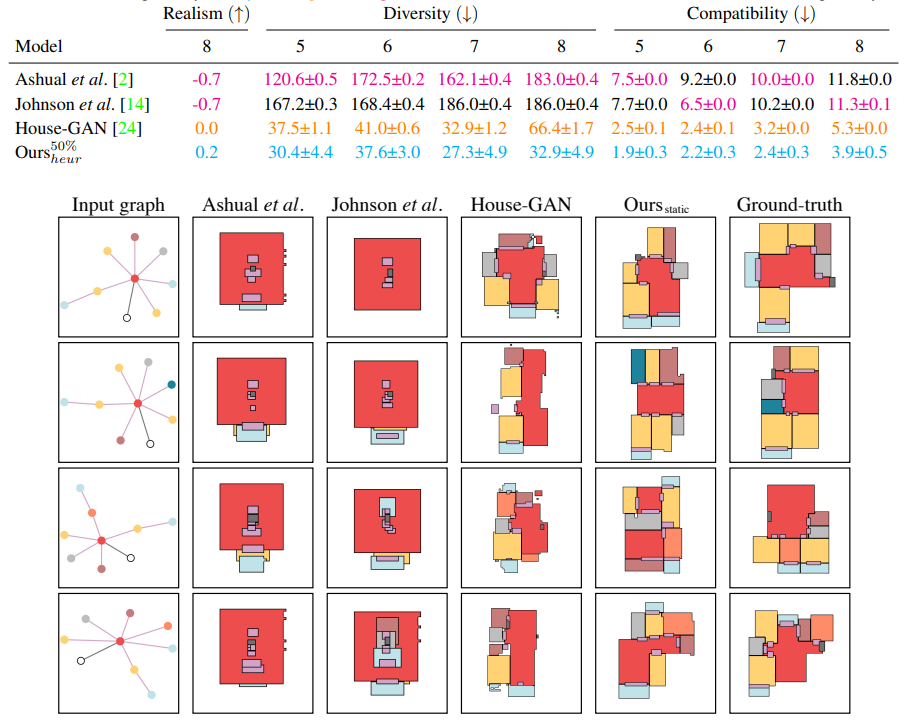
\includegraphics[width=0.8\textwidth]{2/figures/nauata2021_2.png}
		\caption[Evaluación del realismo. Se muestra un diseño generado para cada diagrama de burbujas de entrada]{Evaluación del realismo. Se muestra un diseño generado para cada diagrama de burbujas de entrada.\\
			Fuente: \cite{pr_nauata2021housegan}. \citetitle{pr_nauata2021housegan}. (p. 6)}
		\label{2:fig118}
	\end{center}
\end{figure}

\clearpage
\cite{pr_shen2018localaplognor} publicaron el informe técnico conocido como \citetitle{pr_shen2018localaplognor} en la conferencia "2018 IEEE Wireless Communications and Networking Conference (WCNC)" en Barcelona, España, se presentó el tema "Localización de puntos de acceso basados en el modelo lognormal de Rayleigh".

Este artículo examina el problema de localización de puntos de acceso WiFi (AP) utilizando el modelo Rayleigh lognormal, que caracteriza los efectos del desvanecimiento a gran escala y a pequeña escala. Se propone un método de filtrado de partículas para estimar secuencialmente el alcance de las ubicaciones potenciales del AP objetivo, así como los parámetros de propagación de las señales inalámbricas emitidas por el AP.

El método sugerido se basa en el modelo lognormal de Rayleigh y el filtrado de partículas. El filtrado de partículas reduce gradualmente el alcance de las posibles ubicaciones de un AP objetivo, así como los parámetros de propagación de las señales inalámbricas emitidas por el AP objetivo, cuando un participante que sostiene un smartphone recopila mediciones de intensidad de señal recibida (RSS) de un AP objetivo en posiciones conocidas.

Según experimentos extensos realizados en escenarios típicos de interiores y exteriores, el método sugerido supera a las soluciones basadas en el modelo lognormal en un 14,13\% a 70,38\%. Debido a que las rutas en los dos primeros escenarios están más cerca del AP que en el escenario de oficina, como se muestra en la Figura 11, los errores de localización en los escenarios del centro comercial y la residencia de estudiantes son mucho menores que en el escenario de oficina.

\begin{figure}[!ht]
	\begin{center}
		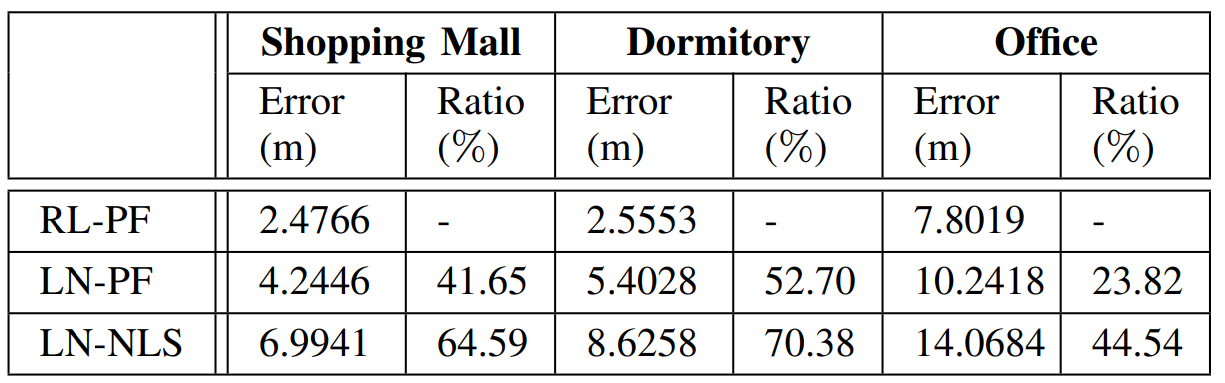
\includegraphics[width=0.75\textwidth]{2/figures/shen2018.png}
		\caption[Comparación de los Errores Medios de Localización en Interiores]{Comparación de los Errores Medios de Localización en Interiores.\\
			Fuente: \cite{pr_shen2018localaplognor}. \citetitle{pr_shen2018localaplognor}. (p. 6)}
		\label{2:fig119}
	\end{center}
\end{figure}

\newpage
\cite{pr_akhter2023interfacesetup} publicó un artículo que se llamaba \citetitle{pr_akhter2023interfacesetup}, "Método de optimización de la configuración de interfaces mediante un modelo de estimación de rendimiento para puntos de acceso que se comunican simultáneamente en una red de área local inalámbrica", según la revista científica "Sensors" de 2023.

La ubicación de los puntos de acceso (AP) en las redes WLAN es crucial para la estimación de la posición de los usuarios en los sistemas de posicionamiento internos. Este ensayo examina cómo la localización de AP afecta la precisión de las estimaciones de ubicación utilizando un método basado en probabilidades. Para evaluar el impacto de la ubicación de los AP en la probabilidad de una estimación correcta, se presentan tanto expresiones analíticas como resultados numéricos.

El artículo describe una técnica para optimizar las interfaces de AP que sigue una serie de pasos importantes. Primero, se enumeran todas las combinaciones posibles de canales CB/no-CB y potencia de transmisión para los AP. Después de elegir una combinación, se estima la RSS requerida, se convierte la RSS estimada en mW y se calculan el SIR individual y el SIR promedio. El proceso se repite hasta encontrar la combinación que proporciona el mayor SIR promedio, lo que determina los canales y potencias de transmisión óptimos para los AP.

Los resultados experimentales muestran que la estimación de SIR puede encontrar la combinación ideal de potencia y tipo de canal que brinda el mayor rendimiento total. Por ejemplo, en la topología 1 con alta interferencia, se observa que la combinación de dos canales CB con potencias de transmisión H y L ofrece el rendimiento total más alto. Por otro lado, en la topología 5 con baja interferencia, la combinación de dos canales CB y un canal no CB con potencias L, L y H proporciona el rendimiento más alto en conjunto. Como se puede ver en la Figura 12, estos resultados se respaldan con valores numéricos que demuestran la eficacia del método sugerido para optimizar la configuración de las interfaces de AP para mejorar el rendimiento de la red WLAN.

\begin{figure}[!ht]
	\begin{center}
		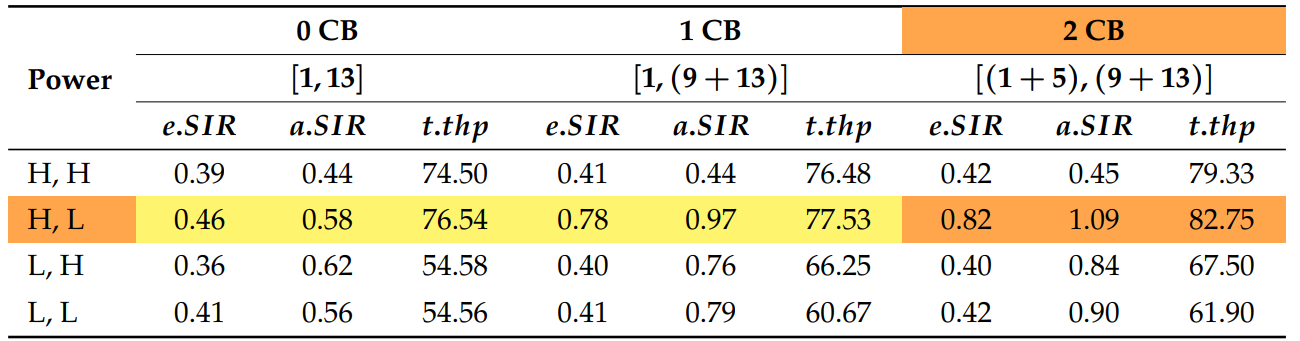
\includegraphics[width=0.75\textwidth]{2/figures/akhter2023.png}
		\caption[Performance estadística del modelo predictivo de los autores]{Performance estadística del modelo predictivo de los autores.\\
		Fuente: \cite{pr_akhter2023interfacesetup}. \citetitle{pr_akhter2023interfacesetup}. (p. 10)}
		\label{2:fig120}
	\end{center}
\end{figure}

\clearpage
\cite{pr_cai2023precisewifi} publicaron un artículo que se llamaba \citetitle{pr_cai2023precisewifi}, el término se traduce al español como "Posicionamiento WiFi preciso en el interior mediante algoritmos de aprendizaje profundo" para la revista científica "ArXiv:2307.02011v" publicada en 2023.

Este artículo presenta una nueva estrategia para el posicionamiento en interiores que emplea tecnología WiFi. Para mejorar la precisión del posicionamiento en comparación con el enfoque tradicional basado únicamente en RSSI, se recomienda utilizar una combinación de mediciones de la Intensidad de la Señal Recibida (RSSI) y el Ángulo de Llegada (AoA).

La metodología se compone de tres pasos principales: 1) Usando puntos de referencia, crear modelos de posicionamiento basados en RSSI y el método híbrido RSSI-AoA; 2) Entrenar los modelos utilizando varios algoritmos de aprendizaje profundo, como BPNN, RBF y CNN; 3) Probar el rendimiento de los modelos y calcular los errores en tres entornos de prueba diferentes: un salón de clases grande, un salón de clases pequeño y un salón de clases pasillo.

Independientemente del algoritmo de aprendizaje profundo utilizado y del entorno de prueba, los resultados muestran que el método híbrido RSSI-AoA tiene un error medio absoluto (MAE) más pequeño que el método basado únicamente en RSSI. Por ejemplo, el MAE del método híbrido con CNN es inferior a 300 mm en un salón de clases grande, mientras que el MAE del método basado en RSSI con CNN es inferior a 400 mm. Como se muestra en la Figura 13, el algoritmo CNN supera a BPNN y RBF en ambos modelos de posicionamiento.

\begin{figure}[!ht]
	\begin{center}
		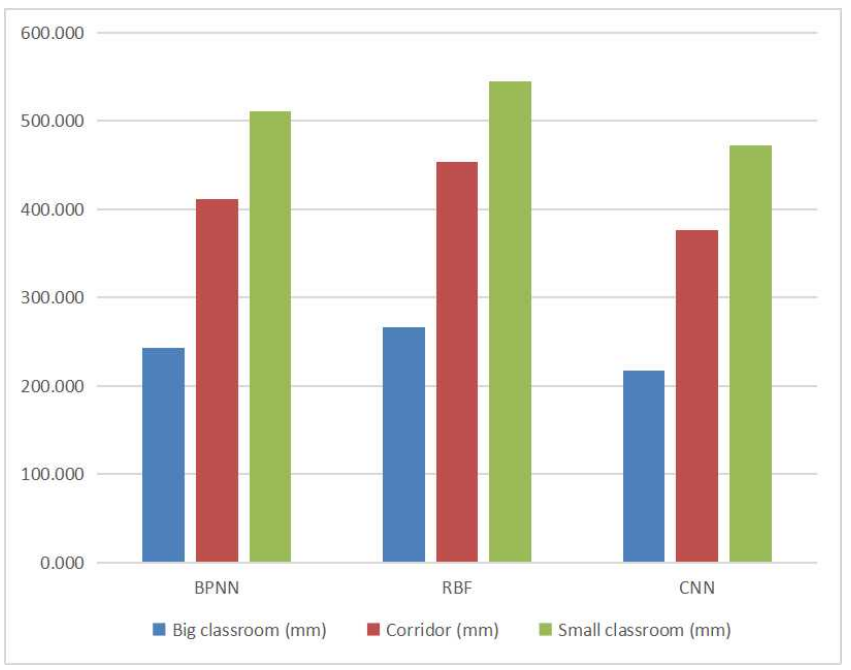
\includegraphics[width=0.90\textwidth]{2/figures/cai2023.png}
		\caption[Los MAE del modelo híbrido de posicionamiento]{Los MAE del modelo híbrido de posicionamiento.\\
			Fuente: \cite{pr_cai2023precisewifi}. \citetitle{pr_cai2023precisewifi}. (p. 26)}
		\label{2:fig121}
	\end{center}
\end{figure}

En el acta de la revista "IPTEK The Journal of Technology and Science", que se llevó a cabo en 2022, se indica que \cite{pr_ainun2022optikmeans} publicaron el artículo conocido como \citetitle{pr_ainun2022optikmeans}, "Optimización de la ubicación de puntos de acceso en redes Wi-Fi utilizando el método de agrupación K-Means", según su traducción al español.

El artículo analiza el uso del algoritmo de agrupamiento K-Means para analizar la fuerza de la señal de cuatro puntos de acceso Wi-Fi en un edificio de dos pisos.

Primero, se realizó un preprocesamiento de datos, que incluyó la eliminación de valores faltantes, eliminación de duplicados y normalización de los datos mediante la normalización Min-Max.  Luego se utilizó el método del codo para encontrar el número ideal de grupos; esto resultó en 4 para el conjunto de datos general y entre 4 y 5 para cada punto de acceso individual.  Posteriormente, con el número de grupos determinado, se utilizó el algoritmo K-Means, lo que resultó en una precisión de entre el 81,5\% y el 83,7\% en la comparación de los valores de BSS y TSS.

Los resultados indican que el grupo con la señal más fuerte para el punto de acceso A tiene una RSSI media de 10,0, mientras que el grupo con la señal más fuerte para el punto de acceso B tiene una RSSI media de 10,5.  Como se muestra en la Figura 14, estos hallazgos podrían ser útiles para maximizar la cobertura de la red Wi-Fi del edificio.

\begin{figure}[!ht]
	\begin{center}
		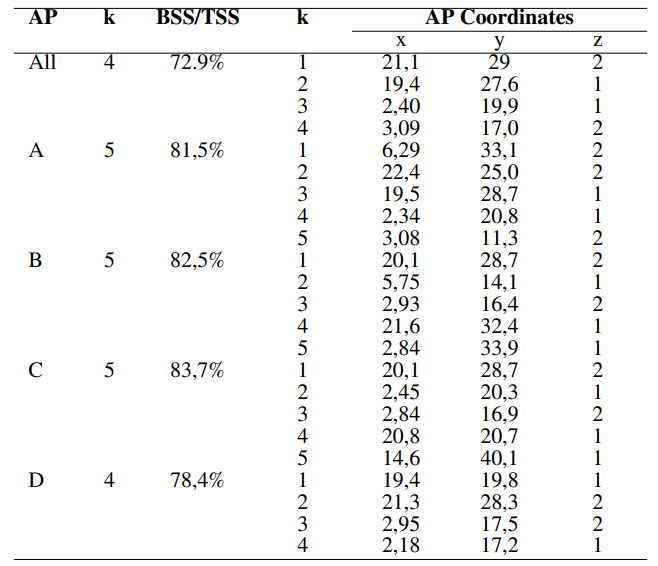
\includegraphics[width=0.65\textwidth]{2/figures/ainun2022.png}
		\caption[Resultados de la aplicación]{Resultados de la aplicación.\\
			Fuente: \cite{pr_ainun2022optikmeans}. \citetitle{pr_ainun2022optikmeans}. (p. 11)}
		\label{2:fig122}
	\end{center}
\end{figure}

\clearpage
En el año 2023, la revista "Automation in Construction" publicó \cite{pr_hosseini2023NSGAIIap} publicaron el artículo conocido como \citetitle{pr_hosseini2023NSGAIIap}, "Ubicación óptima de puntos de acceso Wi-Fi basada en NSGA-II para posicionamiento interior: una predicción RSS basada en BIM", según su traducción al español.

Este artículo presenta un método para optimizar la colocación de puntos de acceso Wi-Fi (AP) en interiores utilizando un modelo de propagación de señal calibrado y un algoritmo genético multiobjetivo (NSGA-II).

La técnica consta de varias etapas: 1) Voxelización del modelo BIM del edificio, 2) Muestreo de intensidad de señal recibida (RSS) en puntos de control y verificación, 3) Calibrar el modelo de propagación de señal mediante el método de cuadrados mínimos, 4) Creación de huellas digitales virtuales 3D y 5) Uso de NSGA-II para optimizar la ubicación de los AP Wi-Fi. 

Los resultados demuestran que el método sugerido puede reducir significativamente el número de AP Wi-Fi necesarios sin sacrificar la precisión de la ubicación. La mejor solución encontrada tenía 4 APs y 13 APs, respectivamente, con una mejora en la precisión del posicionamiento del 35.54\% y 44.82\% en comparación con la distribución actual de 6 APs, como se muestra en la Figura 15.

\begin{figure}[!ht]
	\begin{center}
		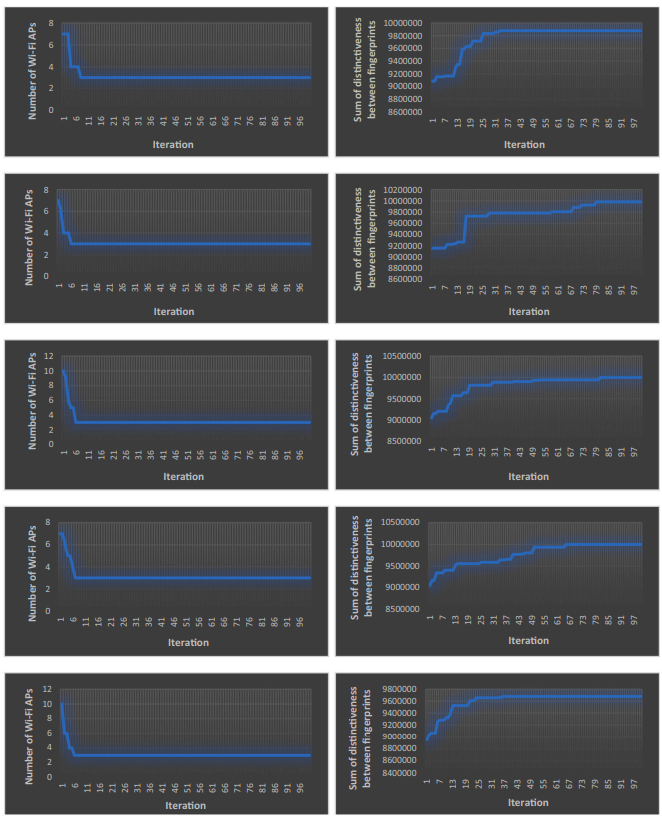
\includegraphics[width=0.75\textwidth]{2/figures/hosseini2023.png}
		\caption[Los resultados de la evaluación de la convergencia del NSGA-II]{Los resultados de la evaluación de la convergencia del NSGA-II.\\
		Fuente: \cite{pr_hosseini2023NSGAIIap}. \citetitle{pr_hosseini2023NSGAIIap}. (p. 16)}
		\label{2:fig123}
	\end{center}
\end{figure}

\newpage
En noviembre del 2015, en la publicación "Computers, Environment and Urban Systems", \cite{pr_lee2015coverage3d} publicaron un artículo que se llamaba \citetitle{pr_lee2015coverage3d}, "Modelización 3D de la ubicación de puntos de acceso Wi-Fi en interiores" en español.

Este documento presenta un modelo de optimización para la ubicación de puntos de acceso (AP) Wi-Fi en un entorno interior de múltiples pisos con el objetivo de maximizar la cobertura de la señal. El modelo utiliza el modelo de sombra log-normal para considerar la atenuación de la señal en tres dimensiones. Esto permite una representación más precisa de la cobertura de la señal en comparación con los métodos tradicionales en dos dimensiones.

El artículo aborda los siguientes puntos importantes: Para estimar la atenuación de la señal en 3D, se define un modelo de propagación de señal log-normal en sombra. El problema de ubicación de AP se identificó como un problema de cobertura de señal máxima (MSCLP), Resolver el MSCLP utilizando un algoritmo de optimización para encontrar las ubicaciones de AP ideales, y finalmente, utilizando esferas que representan la fuerza de la señal en los puntos de demanda para visualizar la cobertura 3D resultante.

El modelo sugerido indica que las ubicaciones de AP ideales se encuentran en varios pisos, con el 70\% de las ubicaciones en los pisos centrales tercero y cuarto. Se logra una cobertura del 98.81\% de los puntos de demanda para una solución con 10 AP sin restricción de capacidad. A medida que se agregan más AP, la fuerza de señal promedio aumenta, pero la tasa de aumento disminuye. La solución propuesta con el mismo número de AP cubre significativamente más puntos de demanda que la solución actual de 117 AP en el edificio de prueba (77.61\% en comparación con 54.63\%). Según el modelo, solo se necesitarían 21 AP sin restricción de capacidad para una cobertura completa, como se muestra en la Figura 16.

\begin{figure}[!ht]
	\begin{center}
		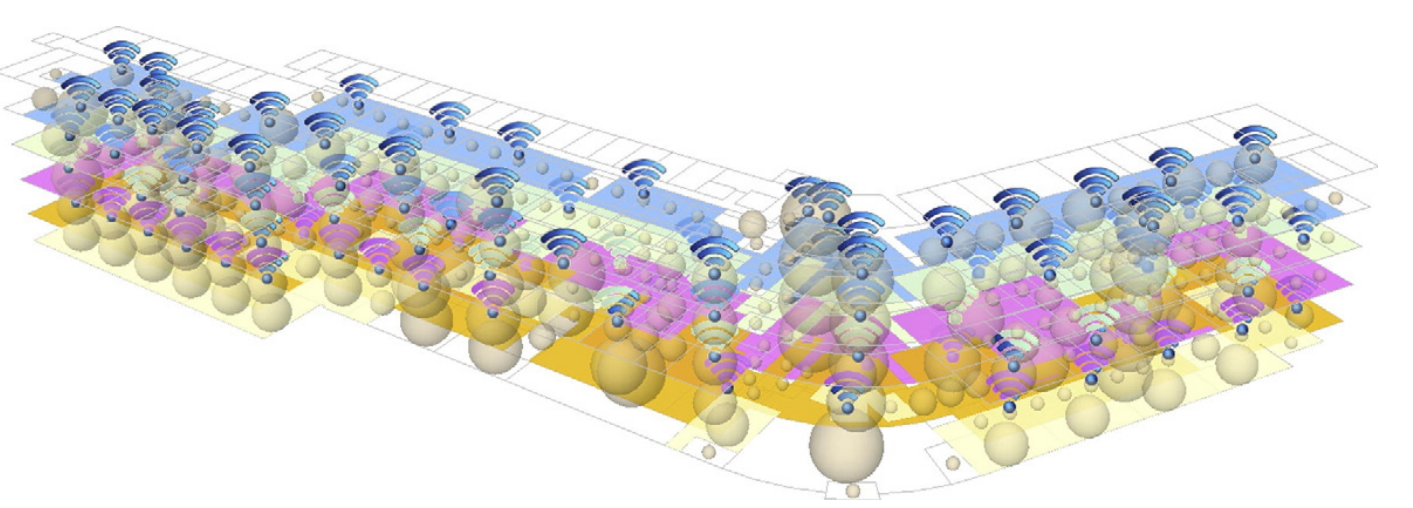
\includegraphics[width=1\textwidth]{2/figures/lee2015.png}
		\caption[Colocación óptima de AP capacitados con demandas ponderadas (p = 117)]{Colocación óptima de AP capacitados con demandas ponderadas (p = 117).\\
		Fuente: \cite{pr_lee2015coverage3d}. \citetitle{pr_lee2015coverage3d}. (p. 9)}
		\label{2:fig124}
	\end{center}
\end{figure}

\newpage
En marzo de 2023, en la revista científica "Architecture and Planning Journal (APJ)", \cite{pr_ozerol2023genermass} publicaron el artículo conocido como \citetitle{pr_ozerol2023genermass}, en español, esto se traduce como "Creación de planes de vivienda colectiva a través de Gans - Un caso en Tokio, Turquía".

El estudio investigó la capacidad de Generative Adversarial Neural Networks (GAN) para crear dibujos arquitectónicos de proyectos de vivienda masiva de TOKI utilizando conjuntos de datos. El objetivo principal fue capacitar al algoritmo HouseGAN para crear tipologías de planos de TOKI actuales y diagramas de burbujas.

En el artículo se explica cómo se multiplicaron planos correlacionados espacialmente con la configuración RGB de 21 tipologías de planos para obtener 157 conjuntos de datos de planos. Estos datos se utilizaron para entrenar al algoritmo de deep learning HouseGAN, que generó imágenes de fondo realistas como salidas del proceso de entrenamiento. El estudio siguió los siguientes pasos: Los diseños arquitectónicos de los proyectos de vivienda masiva de TOKI se utilizaron como conjuntos de datos. Después, se multiplicaron los planos para obtener 157 conjuntos de datos de planos, que se correlacionaron espacialmente con la configuración RGB de 21 tipologías de planos. Posteriormente, se empleó el conjunto de datos generado para entrenar a HouseGAN. Finalmente, los resultados del entrenamiento se convirtieron en imágenes de fondo realistas.

La investigación reveló que la planificación del diseño espacial del algoritmo HouseGAN proporciona diagramas de burbujas y tipologías de planos de TOKI actuales. Como se muestra en la Figura 17, este método permitió crear planos arquitectónicos útiles y realistas para el desarrollo de proyectos de vivienda masiva.

\begin{figure}[!ht]
	\begin{center}
		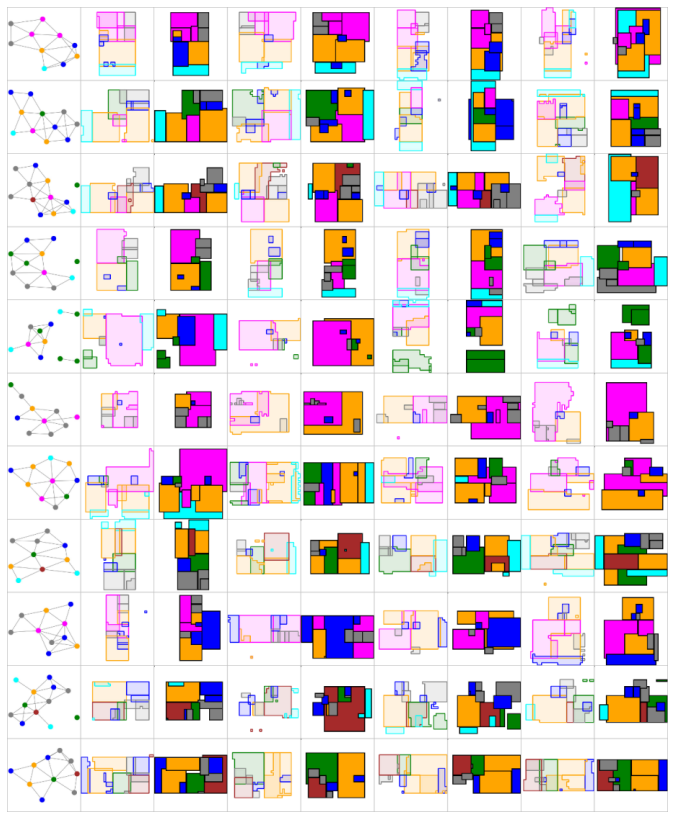
\includegraphics[width=1\textwidth]{2/figures/ozerol2023.png}
		\caption[HouseGAN con LIFULL HOMES Datasets, imágenes generadas por los autores]{HouseGAN con LIFULL HOMES Datasets, imágenes generadas por los autores.\\
		Fuente: \cite{pr_ozerol2023genermass}. \citetitle{pr_ozerol2023genermass}. (p. 10)}
		\label{2:fig125}
	\end{center}
\end{figure}

En marzo del 2023, en la revista "ArXiv", \cite{pr_tang2023graphtransfor} publicaron el artículo conocido como \citetitle{pr_tang2023graphtransfor}, "Transformadores de grafos GAN para la generación de casas con restricciones gráficas" en español.

Los autores de este artículo sugieren una técnica basada en redes generativas adversarias (GAN) con transformadores para crear diseños de casas limitados por un grafo de adyacencia de habitaciones. Mientras que el discriminador clasifica las habitaciones para mantener sus características semánticas, el generador captura las relaciones entre las habitaciones locales y globales utilizando una arquitectura de transformador. Además, se utiliza una pérdida de consistencia cíclica basada en grafos para mantener las relaciones espaciales relativas entre los grafos generados y los reales.

Los siguientes son los pasos principales de la metodología: 1) Representación de entrada: se crea un grafo en el que cada nodo representa una habitación y cada arista representa la proximidad espacial. 2. Red neuronal convolucional de paso de mensaje (Conv-MPN): utiliza transformadores para actualizar los volúmenes de características de las habitaciones y capturar relaciones entre habitaciones conectadas y no conectadas. 3) Discriminador basado en clasificación de nodos: mantiene características semánticas discriminativas importantes para varios elementos de la casa. 4) La pérdida de consistencia cíclica basada en grafos: mantiene las relaciones espaciales relativas entre los grafos generados y los reales.

Los hallazgos demuestran que el enfoque sugerido supera ampliamente a los métodos actuales para generar diseños de casas. En la generación de diseños de techos, GTGAN mejora a los métodos PQ-Net, HouseGAN y RoofGAN con un FID de 9.6 y una distancia mínima de emparejamiento (RMMD) de 7.2 para 4 primitivas. En el subconjunto "10-12" de habitaciones, GTGAN obtiene un puntaje de realismo de 0.25, una distancia FID de 7.5 y una distancia de edición de grafo de 2.63, superando a HouseGAN, HouseGAN++ y otros métodos.

\begin{figure}[!ht]
	\begin{center}
		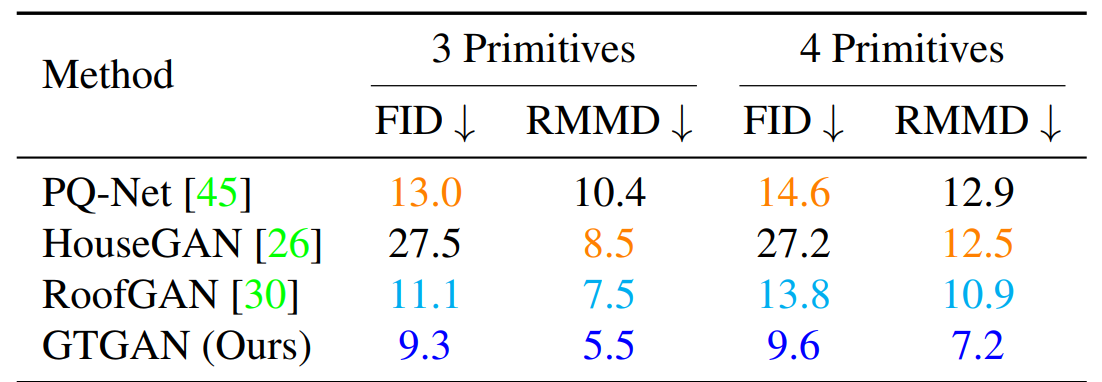
\includegraphics[width=0.65\textwidth]{2/figures/tang2023.png}
		\caption[Resultados cuantitativos de la generación de tejados de casas en el conjunto de datos de geometría de tejados de estilo CAD]{Resultados cuantitativos de la generación de tejados de casas en el conjunto de datos de geometría de tejados de estilo CAD.\\
		Fuente: \cite{pr_tang2023graphtransfor}. \citetitle{pr_tang2023graphtransfor}. (p. 8)}
		\label{2:fig126}
	\end{center}
\end{figure}

\newpage
En abril del 2021, en la revista científica "arXiv", \cite{pr_chang2021buildinggan} publicaron el artículo conocido como \citetitle{pr_chang2021buildinggan}, el título "Building-GAN: generación de diseños arquitectónicos volumétricos condicionados por grafos" se traduce al español.

Para mejorar la eficiencia en el diseño volumétrico de edificios en la industria de la arquitectura y la construcción, este artículo presenta un enfoque innovador llamado Building-GAN. Para visualizar los diseños arquitectónicos, se introduce un grafo de voxels tridimensional, así como un generador que incorpora un módulo de punteros cruzados para conectar el grafo de programas y el grafo de voxels.

El artículo detalla los pasos que se deben seguir para crear el modelo Building-GAN. Comienza con la recopilación de datos, que produce un conjunto de datos sintéticos que incluye 120,000 diseños volumétricos de edificios comerciales. Luego se implementa un Grafo Neural Generativo (GNN) de voxels y se crea un grafo de programas jerárquico. Un módulo cruzado basado en punteros también se agrega para conectar los grafos de programas y los voxels.

Los resultados muestran que el modelo propuesto supera significativamente al método anterior, House-GAN, en un estudio de usuarios con 20 arquitectos profesionales, con una puntuación promedio de 0.85 y 0.92, respectivamente. Además, el modelo propuesto obtiene una puntuación promedio de 0.37 en comparación con el modelo Ground Truth, lo que indica que los arquitectos a menudo no pueden distinguir claramente entre el modelo Ground Truth y el modelo propuesto, como se muestra en la Figura 19.

\begin{figure}[!ht]
	\begin{center}
		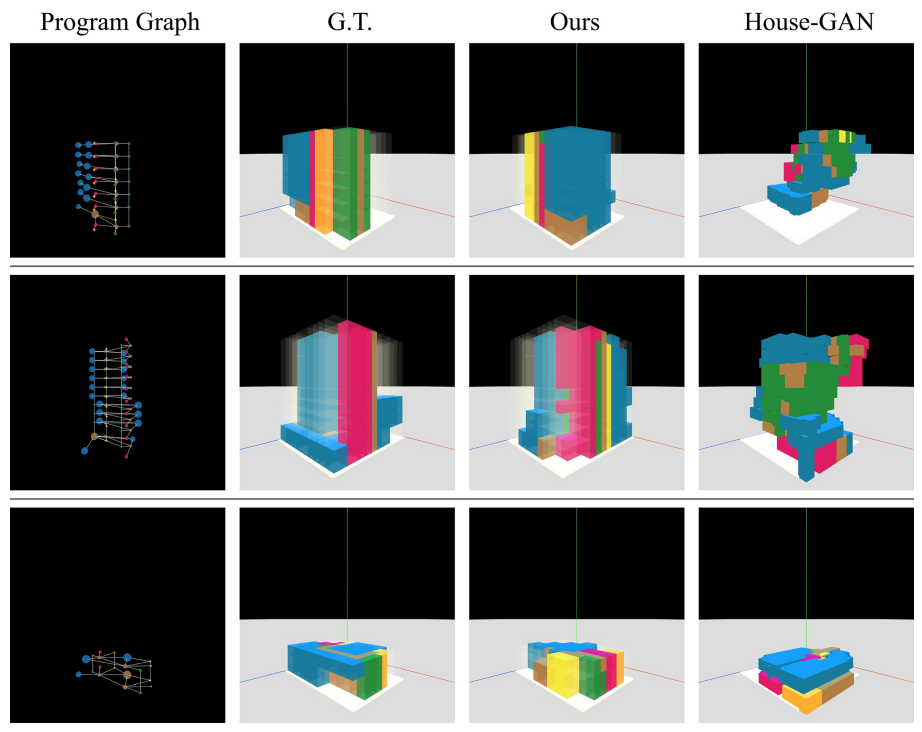
\includegraphics[width=0.7\textwidth]{2/figures/chang2021.png}
		\caption[Para cada gráfico de programa, se generan diseños volumétricos mediante nuestro modelo y mediante House-GAN]{Para cada gráfico de programa, se generan diseños volumétricos mediante nuestro modelo y mediante House-GAN.\\
		Fuente: \cite{pr_chang2021buildinggan}. \citetitle{pr_chang2021buildinggan}. (p. 7)}
		\label{2:fig127}
	\end{center}
\end{figure}

\newpage
\cite{pr_chen2020intelhome3d} publicaron un artículo que se llamaba \citetitle{pr_chen2020intelhome3d}, en español, se ha traducido como "Inteligente Casa 3D: Diseño automático de casas en 3D solo a partir de descripciones lingüísticas" para la revista científica "arXiv" en 2020.

Este artículo presenta un modelo generativo que utiliza descripciones lingüísticas para diseñar automáticamente planos de casas en tres dimensiones. Dos tareas principales componen el proceso: generar el plano de la planta y la síntesis de las texturas internas.

Los siguientes son los pasos que componen la metodología: representar las descripciones lingüísticas en un grafo estructural utilizando un analizador de escenas de Stanford, utilizando una red neuronal condicional de grafos (GC-LPN) para crear un diseño de planta grueso. Refinar el diseño grueso para crear un plano que incluya puertas y ventanas, Usando una red generativa adversaria condicional a lenguaje (LCT-GAN), se pueden sintetizar las texturas interiores de cada habitación. crear y mostrar la escena 3D completa a partir del plano con texturas.

Los hallazgos indican que el 39,41\% de los diseños creados por el modelo no se distinguían de los creados por humanos en un estudio en el que participaron 20 personas. Además, en evaluaciones cuantitativas, el modelo obtuvo un puntaje de IoU de 0,4765 para la generación de planos y un FID de 27,32 para la síntesis de texturas.

\begin{figure}[!ht]
	\begin{center}
		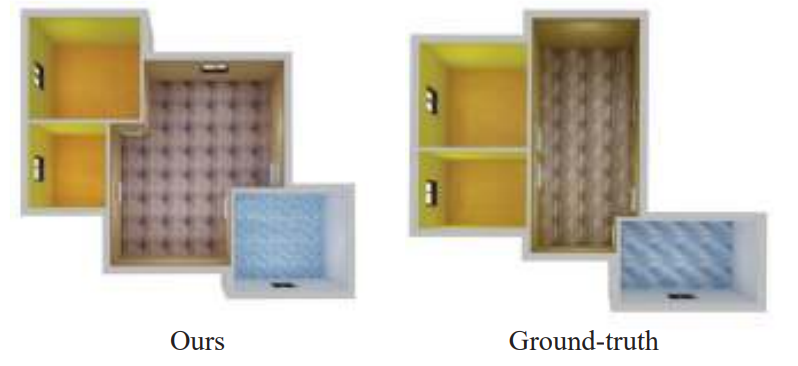
\includegraphics[width=0.73\textwidth]{2/figures/chen2020.png}
		\caption[Comparación de nuestros planos de casas en 3D generados con sus contrapartes reales (hechas por humanos)]{Comparación de nuestros planos de casas en 3D generados con sus contrapartes reales (hechas por humanos).\\
		Fuente: \cite{pr_chen2020intelhome3d}. \citetitle{pr_chen2020intelhome3d}. (p. 8)}
		\label{2:fig128}
	\end{center}
\end{figure}

\newpage
\cite{pr_dou2023researchwir} publicaron un artículo que se llamaba \citetitle{pr_dou2023researchwir}, "Investigación sobre cobertura de red inalámbrica para la transformación y actualización de la gestión expositiva con tecnología de inteligencia artificial", según la revista académica internacional "Matemáticas aplicadas y ciencias no lineales" en junio de 2023.

El rápido crecimiento de la inteligencia artificial y la tecnología de comunicación moderna ofrece una oportunidad poderosa para transformar, actualizar y desarrollar una gestión de exposiciones de alta calidad. Sin embargo, es necesario abordar el problema de la cobertura ideal de la red inalámbrica en el área de exposición. Se ha introducido un nuevo algoritmo de inteligencia artificial basado en la optimización de Harris Hawk (HHO) para abordar este problema.

El artículo resuelve el problema de cobertura de la red inalámbrica utilizando un método de optimización multiobjetivo. Primero, el problema de la cobertura se plantea como una función de objetivo que busca maximizar la cobertura y minimizar la redundancia. Como se muestra en la Figura 21, se resuelve este problema utilizando el algoritmo de optimización de Harris Hawk mejorado (IHHO). El IHHO permite una búsqueda eficiente del espacio de soluciones al simular el comportamiento de los halcones de Harris al cazar presas. Además, para inicializar la población, se utiliza un muestreo de hipercubo latino, lo que mejora la diversidad de la población inicial y reduce la probabilidad de convergencia prematura.

\begin{figure}[!ht]
	\begin{center}
		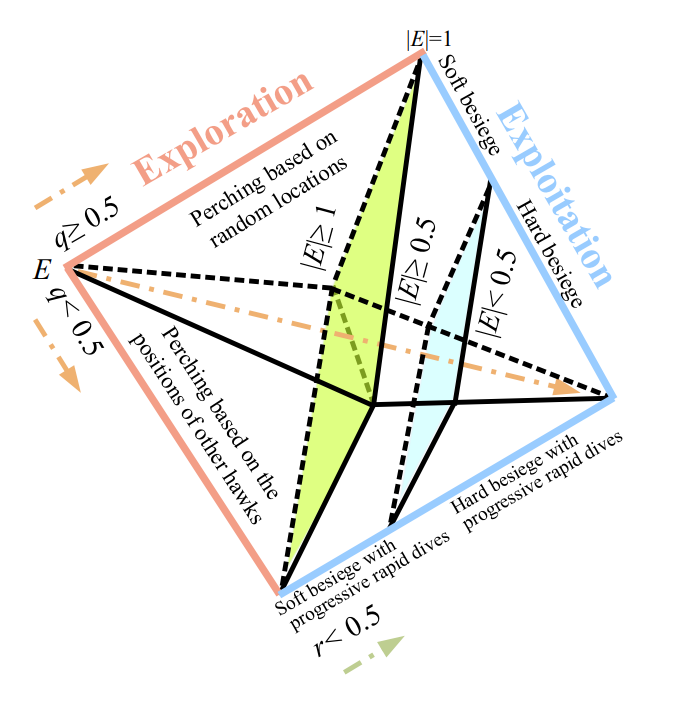
\includegraphics[width=0.70\textwidth]{2/figures/dou2023.png}
		\caption[Estructura de HHO]{Estructura de HHO.\\
		Fuente: \cite{pr_dou2023researchwir}. \citetitle{pr_dou2023researchwir}. (p. 5)}
		\label{2:fig129}
	\end{center}
\end{figure}

\newpage
Como se muestra en la Figura 22, los resultados de la simulación muestran que el algoritmo de optimización tiene un índice de evaluación integral del 98,03\%, que es superior al del optimizador de enjambre de partículas (PSO) y al algoritmo HHO estándar. Esto demuestra que el algoritmo IHHO sugerido es efectivo para resolver los problemas de cobertura de la red inalámbrica y mejora la cobertura de los nodos más que los métodos de optimización convencionales.

\begin{figure}[!ht]
	\begin{center}
		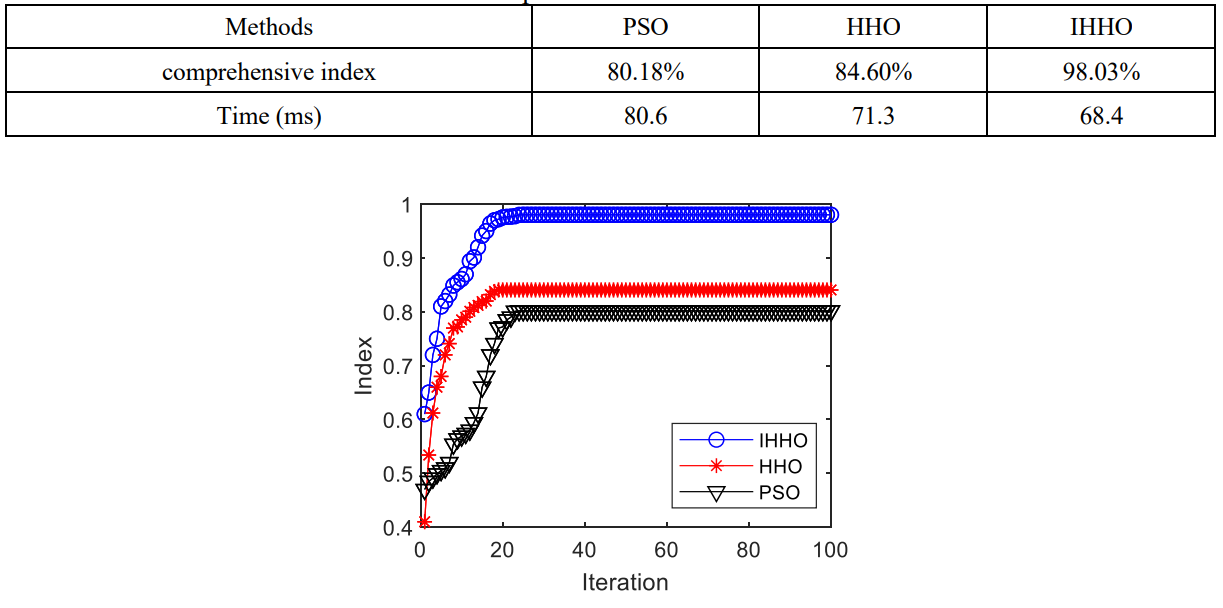
\includegraphics[width=1\textwidth]{2/figures/dou2023_2.png}
		\caption[Comparaciones entre los métodos]{Comparaciones entre los métodos.\\
			Fuente: \cite{pr_dou2023researchwir}. \citetitle{pr_dou2023researchwir}. (p. 11)}
		\label{2:fig130}
	\end{center}
\end{figure}